\documentclass[a4paper,10pt]{article}
\usepackage[utf8]{inputenc}
\usepackage[T1]{fontenc}
\usepackage{lmodern}
\usepackage{graphicx}
\usepackage{tikz}
\usepackage{float}
\usepackage{longtable}
\usepackage{hyperref}
\begin{document}
\begin{titlepage}

\newcommand{\HRule}{\rule{\linewidth}{0.5mm}} % Defines a new command for the horizontal lines, change thickness here

\center % Center everything on the page
 
%----------------------------------------------------------------------------------------
%	HEADING SECTIONS
%----------------------------------------------------------------------------------------

\textsc{\LARGE Université de Mons}\\[1.5cm] % Name of your university/college
\textsc{\Large Compilation }\\[0.5cm] % Major heading such as course name

%----------------------------------------------------------------------------------------
%	TITLE SECTION
%----------------------------------------------------------------------------------------

\HRule \\[0.4cm]
{ \huge \bfseries Implémentation d'un compilateur du language \textrm{Dumbo}}\\[0.4cm] % Title of your document
\HRule \\[1.5cm]
 
%----------------------------------------------------------------------------------------
%	AUTHOR SECTION
%----------------------------------------------------------------------------------------

\begin{minipage}{0.4\textwidth}
\begin{flushleft} \large
\emph{Auteurs :}\\
Florent Delgrange \\
Clément Tamines
\end{flushleft}
\end{minipage}
~
\begin{minipage}{0.4\textwidth}
\begin{flushright} \large
\emph{Professeur:} \\
Véronique Bruyère
\emph{Assistant:} \\
Noémie Meunier
\end{flushright}
\end{minipage}\\[4cm]

% If you don't want a supervisor, uncomment the two lines below and remove the section above
%\Large \emph{Author:}\\
%John \textsc{Smith}\\[3cm] % Your name

%----------------------------------------------------------------------------------------
%	DATE SECTION
%----------------------------------------------------------------------------------------

{\large 23 mai 2016}\\[3cm] % Date, change the \today to a set date if you want to be precise

%----------------------------------------------------------------------------------------
%	LOGO SECTION
%----------------------------------------------------------------------------------------

%\includegraphics{Logo}\\[1cm] % Include a department/university logo - this will require the graphicx package
 
%----------------------------------------------------------------------------------------

\vfill % Fill the rest of the page with whitespace

\end{titlepage}

\newpage
\tableofcontents
\newpage

\section{Introduction}

Le but de ce projet est d'implémenter un compilateur pour le langage \textrm{Dumbo}. Il est demandé d'adapter la grammaire fournie dans l'énoncé pour 
qu'elle gère les expressions arithmétiques, les expressions booléennes ainsi que les structures de contrôle \textbf{if} et les boucles \textbf{for}.
Ce rapport a pout but d'expliquer les techniques que nous avons utilisées afin de réaliser ce compilateur.

\section{Grammaire utilisée}
Afin d'ajouter certaines fonctionnalités, nous avons avons ajouté certaines règles à la grammaire fournie dans l'énoncé.\newline
{\small
< programme > $\rightarrow$ < txt > | < txt > < programme >\\
< programme > $\rightarrow$ < dumbo\_bloc > \\
< programme > $\rightarrow$ < dumbo\_bloc > < programme > \\
< txt > $\rightarrow$ [a-zA-Z0-9; \& <> " - .\textbackslash / \textbackslash n \textbackslash p :, ]+ \\
< dumbo\_bloc > $\rightarrow$ {{ < expressions\_list > }} \\
< expressions\_list > $\rightarrow$ < expression > ; < expressions\_list >\\
< expressions\_list > $\rightarrow$ < expression > ; \\
< expression > $\rightarrow$ print < string\_expression > \\
< expression > $\rightarrow$ for < variable > in < string\_list > do < expressions\_list > endfor \\
< expression > $\rightarrow$ for < variable > in < variable > do < expressions\_list > endfor \\
< expression > $\rightarrow$ if < boolean\_expression > do < expression\_list > endif\\
< expression > $\rightarrow$ < variable > := < string\_expression > \\
< expression > $\rightarrow$ < variable > := < string\_list > \\
< expression > $\rightarrow$ < variable > := < operation > \\
< operation > $\rightarrow$ < integer > \\
< operation > $\rightarrow$ < variable > \\
< operation > $\rightarrow$ < operation > + < operation >\\
< operation > $\rightarrow$ < operation > - < operation >\\
< operation > $\rightarrow$ < operation > * < operation >\\
< operation > $\rightarrow$ < operation > / < operation >\\
< string\_expression > $\rightarrow$ < string > \\
< string\_expression > $\rightarrow$ < variable > \\
< string\_expression > $\rightarrow$ < string\_expression > . < string\_expression > \\
< string\_list > $\rightarrow$ ( < string\_list\_interior > ) \\
< string\_list\_interior > $\rightarrow$ < string >\\
< string\_list\_interior > $\rightarrow$ < string >, < string\_list\_interior > \\
< boolean\_expression > $\rightarrow$ < boolean > \\
< boolean\_expression > $\rightarrow$ < boolean\_expression > and < boolean\_expression > \\
< boolean\_expression > $\rightarrow$ < boolean\_expression > or < boolean\_expression > \\
< boolean\_expression > $\rightarrow$ < variable > < < variable >\\
< boolean\_expression > $\rightarrow$ < variable > > < variable >\\
< boolean\_expression > $\rightarrow$ < variable > = < variable >\\
< boolean\_expression > $\rightarrow$ < variable > != < variable >\\
< boolean > $\rightarrow$ [true|false]\\
< integer > $\rightarrow$ \textbackslash d+\\
< variable > $\rightarrow$ [a-z|A-Z]+[a-z|A-Z|0-9\_]*\\
< string > $\rightarrow$ '[a-zA-Z0-9; \& <> " - .\textbackslash / \textbackslash n\textbackslash p :, =]+' \\
}

Nous avons tout d'abord ajouté les règles < operation > qui permettent de stocker des entiers dans des variables : celles-ci contiennent donc des entiers ou bien le résultat
de calculs sur des entiers. Nous avons ensuite ajouté les expressions booléennes. Celles-ci sont utilisées comme conditions dans 
le \textrm{if}.\\
Une expression booléenne peut être \textrm{true} ou \textrm{false} et peut aussi être le résultat d'une comparaison de deux entiers contenus dans des variables. Nous permettons d'effectuer des tests \textrm{or} et \textrm{and} entre plusieurs expressions booléennes.

Cette grammaire ainsi modifiée ne nous permet cependant pas certaines fonctionnalités, qui n'étaient pas expressément demandées dans l'énoncé :
\begin{itemize}
 \item Nous ne permettons pas de stocker des valeurs booléennes dans des variables, ces expressions étant seulement utilisées par la structure de contrôle \textrm{if}. 
 \item Nous ne permettons pas les comparaisons entre entiers et variables ou entre entiers. Lors des comparaisons, seules des entiers contenus dans des variables
 peuvent être utilisés.
\end{itemize}


\section{Arbre de dérivation}
Lors de l'analyse syntaxique, un arbre de dérivation est créé. Une fois une règle de la grammaire détectée, un noeud spécial correspondant à cette règle est
créé. Chaque nœud peut posséder ou non des fils et son exécution peut résulter en un comportement différent. Nous obtenons à la fin de l'analyse syntaxique un arbre de dérivation. La racine de l'arbre ainsi créé est 
retourné lorsque l'analyse syntaxique est terminée. Pour exécuter le code contenu dans l'arbre il ne nous reste plus qu'à demander l'exécution de l'arbre, 
ce qui se fait en appelant la méthode \textrm{ex()} sur la racine. Celle-ci va alors récursivement appeller cette méthode sur ses fils et récupérer le résultat 
de leur exécution ce qui nous donnera le résultat de l'exécution du programme entier. Nous avons illustré ce principe via l'exemple de programme suivant : \\
\begin{verbatim}
<html>
{{
    print 'mot1'.'mot2';
}}
</html>
\end{verbatim}

Lorsque nous appliquerons notre analyseur syntaxique sur ce code, l'arbre suivant sera produit (cet arbre est une version simplifiée) :

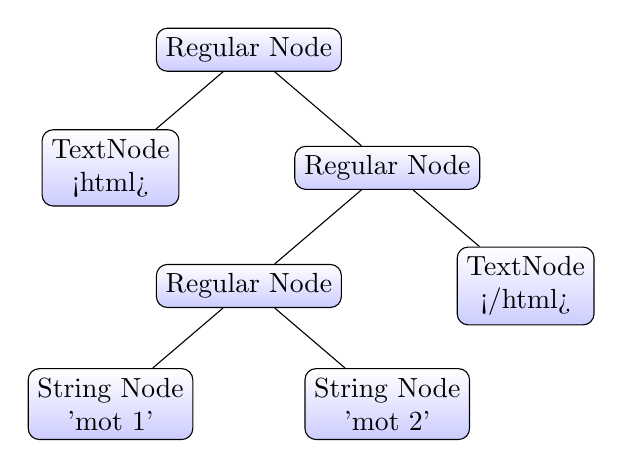
\begin{tikzpicture}[sibling distance=10em,
  every node/.style = {shape=rectangle, rounded corners,
    draw, align=center,
    top color=white, bottom color=blue!20}]]
    \node {Regular Node}
    child { node  {TextNode \\ <html>} }
    child{ node {Regular Node}
        child { node {Regular Node}
            child { node{String Node \\ 'mot 1'} }
            child { node{String Node \\ 'mot 2'} }
        }
        child { node{TextNode \\ </html>} }
    };
\end{tikzpicture}

Appliquer \textrm{ex()} sur la racine de cet arbre pour exécuter le programme qu'il représente va avoir le comportement suivant : \\
La racine va demander le résultat de l'exécution de son premier fils, celui-ci étant un nœud texte, il va renvoyer le texte qu'il contient. Le résultat du deuxième fils sera alors
demandé, récursivement ce nœud va demander le résultat de son premier fils, qui renverra la chaine de caractère \textrm{mot1} qu'il contient sans les \textbf{'}. Ceci est le comportement
spécifique aux nœuds stockant les chaines de caractère. Il en sera de même pour son fils droit qui renverra \textrm{mot2}. Le père contiendra alors la chaine de
caractère \textrm{mot1mot2} qu'il renverra à son propre père. Celui-ci va demander l'exécution de son deuxième fils, qui est un noeud texte renvoyant \textrm{<\textbackslash html>}
La racine possédant alors le résultat de l'exécution de tout ses fils, elle met ensemble ces résultats et renvoie la valeur obtenue. Cette valeur correspond au résultat de 
l'exécution du programme contenu dans l'arbre.\\

En résumé, chaque nœud de l'arbre construit a une fonction spécifique et renverra le résultat de son exécution sous forme d'une chaine de caractère.
Certains nœuds ont une fonction particulière qui ne renvoie aucune donnée. C'est le cas des nœuds d'assignation qui servent juste à ajouter une valeur dans le dictionnaire qui sert de 
table de variables (chaque variable étant une paire clé-valeur). Ce nœud, lorsqu'il est exécuté, se contente d'ajouter dans la table la clé qu'il contient et d'y associer la valeur demandée
par l'assignation (cette valeur résulte de l'exécution d'un autre nœud, par exemple d'un nœud réalisant des opérations arithmétiques). \\
Ajouter une règle à la grammaire est alors facile puisqu'il suffira de créer un nœud qui gèrera le comportement voulu lors de la détection de cette règle. 

\section{Gestion du \textbf{if} et \textbf{for}}
Pour implémenter la structure de contrôle \textrm{if}, nous avons tout d'abord ajoutés les lexèmes \textbf{if} et \textbf{endif} dans l'analyseur lexical. Nous avons ensuite ajouté la 
règle suivante à la grammaire : < expression > $\rightarrow$ if < boolean\_expression > do < expression\_list > endif. \\
Lorsque cette règle est détectée par l'interpréteur, un nœud gérant le if est créé. Il possède une référence au nœud contenant la condition booléenne et une référence au nœud qui correspond
à l'action à effectuer si cette condition est vérifiée. Lors de l'exécution du nœud \textrm{if}, nous exécutons le nœud qui contient la condition booléenne. Le résultat de cette exécution
est récupéré et si la condition était vérifiée (\textrm{True} est renvoyé) alors nous exécutons le nœud contenant l'action à effectuer et le résultat de cette exécution est renvoyé. \\
Au final, à la fin de l'exécution du nœud, une chaine de caractère est renvoyée et celle-ci contient soit le résultat de l'exécution de l'action du if si la condition était vraie, soit une
chaine de caractères vide si la condition était fausse. 
\newline
Le nœud gérant le \textrm{if} est implémenté de la manière suivante : \\
\begin{verbatim}

class IfNode():
   def __init__(self, *args):
      #Le nœud prend en paramètre les nœuds contenant la condition et l'action du if, dans l'ordre fourni par la règle
      self.sons = args
         
   def ex(self):
      condition = self.sons[0]
      action = self.sons[1]

      res = "" #Le résultat est une chaine vide, sauf si la condition est vraie
      if(condition.ex()):
         res += str(action.ex()) #Si l'exécution du nœud contenant la condition est vraie, nous exécutons le nœud contenant l'action
      return res
 
\end{verbatim}

Le \textrm{for} est créé avec la même logique que le \textrm{if}. Une fois une règle pour le \textrm{for} détectée, un nœud spécial est créé. Celui-ci prend en paramètre le nœud contenant
la variable, le nœud contenant la liste et le nœud contenant l'action à effectuer. Nous commençons d'abord par vérifier que la variable utilisée dans le for n'existe pas déjà dans la 
table des symboles. Si elle existe déjà, nous retenons sa valeur initiale pour la réassigner à la fin de la boucle. Nous récupérons ensuite la liste d'éléments contenue dans un nœud de variable
ou dans un nœud de liste via son exécution. Nous remarquons ici l'utilité d'avoir des nœuds différents implémentant chacun leur propre manière de s'exécuter. Si une variable contenant
une liste a été fournie, l'exécution du nœud contenant cette variable renverra la valeur associée au nom de la variable dans la table de variables. Si une liste a été directement fournie,
l'exécution du nœud renverra simplement cette liste. Cette méthode nous permet de ne pas faire la différence entre une liste contenue dans une variable ou une liste donnée directement. L'exécution
du nœud renverra une liste indépendamment de son type. Il nous suffit ensuite de parcourir chaque élément de la liste, d'assigner à la variable la valeur de l'élément courant dans la table
des variables et d'effectuer l'action via l'exécution du nœud la contenant. Le résultat de cette exécution est récupéré dans une chaine de caractères et sera renvoyé une fois la boucle 
terminée. Il ne nous reste enfin qu'à rendre à la variable sa valeur initiale si elle en avait une et de renvoyer le résultat de l'exécution de la boucle.
\begin{verbatim}
 class ForNode():
   def __init__(self, *args):
      self.sons = args
         
   def ex(self):
      var_name = str(self.sons[0]) #Nom de la variable

      initial_value = "" #Valeur initiale de la variable

      #Si la variable éxiste déjà et a une valeur, nous la retenons
      if var_name in variables:
         initial_value = variables[var_name]

      list_or_var = self.sons[1].ex() #Récupérons le contenu de la var ou de la liste
      
      action = self.sons[2]
      res = ""
      for var in list_or_var:
         variables[var_name] = var
         res+=action.ex()

      #Si la variable avait une valeur initiale, nous la réinstallons
      if initial_value != "":
         variables[var_name] = initial_value

      return res
\end{verbatim}

\section{Difficultés rencontrées}

\subsection{Mauvaise détection des lexèmes}
Lors de nos tests, nous nous sommes rendus compte que l'analyseur lexical détectait mal certains lexèmes. Tout d'abord, le lexème texte était parfois détecté comme un lexème de variable
et vice-versa. La solution que nous avons trouvée a été de créer deux états dans l'analyseur lexical, l'un pour détecter des lexèmes lorsque nous étions hors d'un dumbo bloc 
contenant du code Dumbo et l'autre lorsque nous étions dans un dumbo bloc. Nous avons appelé cet état inBlock. Hors de cet état, seul le lexème texte peut être détecté. 
Lorsque le lexème HOOK\_OPEN signifiant l'entrée dans un dumbo bloc est rencontré, l'analyseur lexical entre dans l'état inBlock et seul les mots clés ainsi que les variables, entiers et 
chaines de caractères peuvent être détectés. L'analyseur ne pourra pas confondre les lexèmes texte et variables car chacun de ces lexèmes appartient à un état différent et l'analyseur 
ne peut détecter qu'un seul de ces lexèmes selon l'état dans lequel il se trouve. \\
L'autre problème que nous avons rencontré est le suivant : dans l'état inBlock nous avons remarqué que les symboles réservés du langage ainsi que les nombres entiers 
étaient détectés comme des noms de variables dans certains cas. En effet le lexème variable étant le premier décrit dans cet état, lorsque l'analyseur rencontrait un \textrm{if} celui-ci 
était détecté comme une variable et rendait l'exécution impossible. Il en est de même pour \textrm{or}, \textrm{and}, ect. Nous avons réglé ce problème via l'utilisation d'un dictionnaire
de mots réservés dans le langage. Lorsque \textrm{if} est détecté comme une variable, ce dictionnaire est consulté avec \textrm{if} comme clé. Si if faisait partie du dictionnaire 
alors nous savons que c'est un mot réservé, la valeur correspondant à \textrm{if} dans le dictionnaire est le type correct de lexème à associer à \textrm{if}. Ceci n'empêche pas la détection
de mots réservés comme lexèmes de type variable mais corrige leur type lorsque cette mauvaise détection arrive.\\
En ce qui concerne les nombres entiers, nous avons empêché les noms de variables de commencer par un entier. Ceci empêche les entiers d'être confondus avec des noms de variable. 
Cette restriction ne nous a pas paru mauvaise car elle se fait dans de nombreux autres langages de programmation.

\end{document}
